\documentclass[]{article}
\usepackage[T1]{fontenc}
\usepackage[english]{babel}
\usepackage[utf8]{inputenc}
\usepackage{color}
\usepackage{listings}
\usepackage{courier}
\usepackage{cite}
\usepackage{graphicx}
\usepackage{hyperref}
\usepackage[xindy]{glossaries}
\makeglossaries

\newacronym{dac}{DAC}{Discretionary Access Control}
\newacronym{mac}{MAC}{Mandatory Access Control}
\newacronym{nsa}{NSA}{National Security Agency}
\newacronym{sel}{SELinux}{Security-Enhanced Linux}
\newacronym{dte}{DTE}{Domain and Type Enforcement}
\newacronym{lids}{LIDS}{Linux Intrusion Detection System}
\newacronym{lsm}{LSM}{Linux Security Modules}

\lstset{ %
language=C,                % choose the language of the code
basicstyle=\footnotesize\ttfamily,       % the size of the fonts that are used for the code
numbers=left,                   % where to put the line-numbers
numberstyle=\footnotesize,      % the size of the fonts that are used for the line-numbers
stepnumber=1,                   % the step between two line-numbers. If it is 1 each line will be numbered
numbersep=5pt,                  % how far the line-numbers are from the code
backgroundcolor=\color{white},  % choose the background color. You must add \usepackage{color}
showspaces=false,               % show spaces adding particular underscores
showstringspaces=false,         % underline spaces within strings
showtabs=false,                 % show tabs within strings adding particular underscores
frame=bt,           % adds a frame around the code
tabsize=2,          % sets default tabsize to 2 spaces
captionpos=b,           % sets the caption-position to bottom
breaklines=true,        % sets automatic line breaking
breakatwhitespace=false    % sets if automatic breaks should only happen at whitespace
}


\begin{document}

\title{Introduction to Linux Security Modules\\ \small{Draft}}
%\subtitle{}
\author{Rui Gonçalo
        \\{\scriptsize \texttt{pg18378@alunos.uminho.pt}}
       }
\date{\today}
\maketitle

\begin{abstract}
``If you cannot explain it simply, you do not understand it well enough.''
\end{abstract}


\section{Introduction}
Introduction

\section{Motivation}
\label{sec:motivation}

DroidGuardian aims to provide a fine-grained control over internet connections on Android devices. This feature allows users to be aware of how applications behave in terms of outgoing connections that usually occur hidden and unnoticed. Most of the times it is supposed to be like that. Internet connections are a mean to get and send data, quickly, secretly and efficiently. However, the user, as the device's owner, should know what is going under the hood if he desires to. Should be able to find out what connections are applications that live inside his device doing.

%\begin{itemize}
%\item Describe the relevance of Android in the smartphone global market;
%\item Substantiate with real numbers extracted from available reports;
%\item Introduce the associated risks with the popularity of Android;
%\item Explain why is important to invest in Android OS security.
%\end{itemize}

\section{Objectives}
\label{sec:objectives}

%Define objectives and a brief explanation on how they will be accomplished.

\section{Structure}

%Structure of the dissertation.

\section{Design}
The basic abstraction of the \gls{lsm} interface is to intercede in the access to internal kernel objects. Security modules should answer a simple question "May a subject \texttt{S} perform a kernel operation \texttt{OP} on an internal kernel object \texttt{OBJ}?". The mechanism that allow modules to execute this task lies in \textit{hook} functions that are placed in the kernel code, as shown in \autoref{fig:lsm_arch}.

\begin{figure}[htbp]
 \centering
 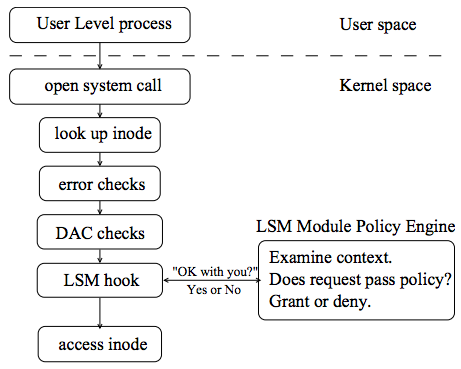
\includegraphics[scale=0.5]{images/LSM_architecture.png}
 \caption{LSM hook functions architecture}
 \label{fig:lsm_arch}
\end{figure}

\noindent
Immediately before the kernel access the object, represented as \textit{inode} in \autoref{fig:lsm_arch}, the hook makes a call to a function that the \gls{lsm} must provide. The module, based on policy rules, either allow or deny the access, forcing an error code return in the last case.


\section{Implementation}
The \gls{lsm} framework comprises a few files in the kernel. \autoref{fig:kernel_files} highlights the relevant files that implement the security mechanism.

\begin{figure}[htbp]
 \centering
 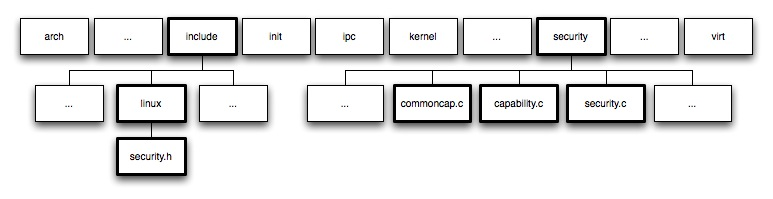
\includegraphics[scale=0.5]{images/kernel_files.jpg}
 \caption{\gls{lsm} framework files in the Linux kernel}
 \label{fig:kernel_files}
\end{figure}

\subsection{Header file}
\label{sec:header_file}

The \texttt{include/linux/security.h} file contains the hook functions declarations. The source code may be divided into two parts, depending on the value of the conditional group \texttt{CONFIG\_SECURITY} being true or false. In the first case, an extensive structure with pointers to all hook functions is declared. If false, only default functions are declared and the kernel loads the default security module. The code snippet in \autoref{lst:struct_ops}, extracted from the Linux kernel v3.11, presents the initial function pointers in the structure \texttt{security\_operations}.

\begin{lstlisting}[frame=none, numbers=none, caption=Security structure declaration (Linux kernel v3.11), label=lst:struct_ops]
struct security_operations {
	char name[SECURITY_NAME_MAX + 1];

	int (*ptrace_access_check) (struct task_struct *child, unsigned int mode);
	int (*ptrace_traceme) (struct task_struct *parent);
	int (*capget) (struct task_struct *target,
		       kernel_cap_t *effective,
		       kernel_cap_t *inheritable, kernel_cap_t *permitted);
	int (*capset) (struct cred *new,
		       const struct cred *old,
		       const kernel_cap_t *effective,
		       const kernel_cap_t *inheritable,
		       const kernel_cap_t *permitted);
	int (*capable) (const struct cred *cred, struct user_namespace *ns,
			int cap, int audit);
	int (*quotactl) (int cmds, int type, int id, struct super_block *sb);
	int (*quota_on) (struct dentry *dentry);
	int (*syslog) (int type);
	int (*settime) (const struct timespec *ts, const struct timezone *tz);
	int (*vm_enough_memory) (struct mm_struct *mm, long pages);
\end{lstlisting}

\noindent
Along with the structure, the functions prototypes are declared, as shown in \autoref{lst:hooks}. Some security hooks are declared depending on conditional groups:

\begin{itemize}
 \item \texttt{CONFIG\_SECURITY\_PATH}, includes security hooks for pathname based access control;
 \item \texttt{CONFIG\_SECURITY\_NETWORK}, enables socket and network security hooks;
 \item \texttt{CONFIG\_SECURITY\_NETWORK\_XFRM}, security hooks for XFRM framework, that implement per-packet access controls based on labels derived from IPSec policy;
\item \texttt{CONFIG\_KEYS}, provides support for retaining authentication tokens and access keys in the kernel;
\item \texttt{CONFIG\_AUDIT}, enables auditing infrastructure that can be used with another kernel subsystem.
\end{itemize}

\begin{lstlisting}[frame=none, numbers=none, caption=Security functions declaration (Linux kernel v3.11), label=lst:hooks]
int security_ptrace_access_check(struct task_struct *child, unsigned int mode);
int security_ptrace_traceme(struct task_struct *parent);
int security_capget(struct task_struct *target,
		    kernel_cap_t *effective,
		    kernel_cap_t *inheritable,
		    kernel_cap_t *permitted);
int security_capset(struct cred *new, const struct cred *old,
		    const kernel_cap_t *effective,
		    const kernel_cap_t *inheritable,
		    const kernel_cap_t *permitted);
int security_capable(const struct cred *cred, struct user_namespace *ns,
			int cap);
int security_capable_noaudit(const struct cred *cred, struct user_namespace *ns,
			     int cap);
int security_quotactl(int cmds, int type, int id, struct super_block *sb);
int security_quota_on(struct dentry *dentry);
int security_syslog(int type);
int security_settime(const struct timespec *ts, const struct timezone *tz);
int security_vm_enough_memory_mm(struct mm_struct *mm, long pages);
\end{lstlisting}

\noindent
If the configurable option \texttt{CONFIG\_SECURITY} is not selected, the default security module is loaded. This module only executes a few capabilities, being permissive in all other hooks, which means that allow access to all kernel internal objects. \autoref{lst:default_hooks} exhibits some of these hooks' source code.

\begin{lstlisting}[frame=none, numbers=none, caption=Default security functions (Linux kernel v3.11), label=lst:default_hooks]
static inline int security_capable(const struct cred *cred,
				   struct user_namespace *ns, int cap)
{
	return cap_capable(cred, ns, cap, SECURITY_CAP_AUDIT);
}

static inline int security_capable_noaudit(const struct cred *cred,
					   struct user_namespace *ns, int cap) {
	return cap_capable(cred, ns, cap, SECURITY_CAP_NOAUDIT);
}

static inline int security_quotactl(int cmds, int type, int id,
				     struct super_block *sb)
{
	return 0;
}

static inline int security_quota_on(struct dentry *dentry)
{
	return 0;
}

static inline int security_syslog(int type)
{
	return 0;
}
\end{lstlisting}

\noindent
The same process is kept to the other configurable options. Depending on their values, security hooks are either declared or coded with default instructions.

\subsection{Linux capabilities}
\label{sec:linux_capabilities}

Linux capabilities were designed to provide a solution to the UNIX-style user privilege set composed by privilege users (\texttt{root}) and non-privilege users \texttt{regular user}. The first type has permission to execute every operation and the former can only execute a few set of operations. Thus, processes run either with all permissions or with very restrictive permissions. Unfortunately, most of the time processes do not need all privileges and this exposure raises serious risk when a process gets compromised \cite{Wiki:Capabilities}.\\

\noindent
In the scope of \gls{lsm}, a set of functions called common capabilities were developed to give the security framework a default behavior in the case no other \gls{lsm} is loaded. These functions are plugged in the kernel to overcome the privilege problem mentioned above. In \texttt{security/commoncap.c} we can see the source code of these functions.\\

\noindent
If no \gls{lsm} is loaded, there must be a default function hook that does not execute any operation and let the process access kernel internal objects. The file \texttt{security/capability.c} have all hook functions with the default code. If the return type is \texttt{void}, functions have no operations, otherwise is \texttt{int} and functions just \texttt{return 0}, which is the value to turn the hook permissive. \autoref{lst:cap_hooks} shows some of these hook functions.

\begin{lstlisting}[frame=none, numbers=none, caption=Capability functions (Linux kernel v3.11), label=lst:cap_hooks]
static int cap_syslog(int type)
{
	return 0;
}

static int cap_quotactl(int cmds, int type, int id, struct super_block *sb)
{
	return 0;
}

static int cap_quota_on(struct dentry *dentry)
{
	return 0;
}

static int cap_bprm_check_security(struct linux_binprm *bprm)
{
	return 0;
}

static void cap_bprm_committing_creds(struct linux_binprm *bprm)
{
}
\end{lstlisting}

\noindent
These functions are called in the structure \texttt{security\_operations} if the respective hook functions are not declared. \autoref{lst:fixup_ops} presents the code snippet of the function \texttt{security\_fixup\_ops}.

\begin{lstlisting}[frame=none, numbers=none, caption=\texttt{security\_fixup\_ops} function (Linux kernel v3.11), label=lst:fixup_ops]
#define set_to_cap_if_null(ops, function)				\
	do {								\
		if (!ops->function) {					\
			ops->function = cap_##function;			\
			pr_debug("Had to override the " #function	\
				 " security operation with the default.\n");\
			}						\
	} while (0)

void __init security_fixup_ops(struct security_operations *ops)
{
	set_to_cap_if_null(ops, ptrace_access_check);
	set_to_cap_if_null(ops, ptrace_traceme);
	set_to_cap_if_null(ops, capget);
	set_to_cap_if_null(ops, capset);
	set_to_cap_if_null(ops, capable);
	set_to_cap_if_null(ops, quotactl);
	set_to_cap_if_null(ops, quota_on);
	set_to_cap_if_null(ops, syslog);
	set_to_cap_if_null(ops, settime);
	set_to_cap_if_null(ops, vm_enough_memory);
(...)
}
\end{lstlisting}

\subsection{Framework initialization}
\label{sec:framework_initialization}

The header file mentioned in \autoref{sec:header_file} declares some functions in charge of getting the \gls{lsm} loaded, as shown in \autoref{lst:init_functions}.

\begin{lstlisting}[frame=none, numbers=none, caption=Framework initialization functions (Linux kernel v3.11), label=lst:init_functions]
/* prototypes */
extern int security_init(void);
extern int security_module_enable(struct security_operations *ops);
extern int register_security(struct security_operations *ops);
extern void __init security_fixup_ops(struct security_operations *ops);
\end{lstlisting}

\noindent
These functions are implemented in \texttt{security/security.c}. The first function being executed is \texttt{security\_init}, which source code is present in \autoref{lst:security_init_func}.

\begin{lstlisting}[frame=none, numbers=none, caption=\texttt{security\_init} function (Linux kernel v3.11), label=lst:security_init_func]
/* Boot-time LSM user choice */
static __initdata char chosen_lsm[SECURITY_NAME_MAX + 1] =
	CONFIG_DEFAULT_SECURITY;

static struct security_operations *security_ops;
static struct security_operations default_security_ops = {
	.name	= "default",
};

(...)

int __init security_init(void)
{
	printk(KERN_INFO "Security Framework initialized\n");

	security_fixup_ops(&default_security_ops);
	security_ops = &default_security_ops;
	do_security_initcalls();

	return 0;
}
\end{lstlisting}

\noindent
At first, the default module is loaded with the available routines cited in \autoref{sec:linux_capabilities}, by \texttt{security\_fixup\_ops(&default\_security\_ops)}. Then \texttt{security\_init()} updates the kernel's security structure \texttt{security\_ops} with the initialized earlier and makes a call to \texttt{do\_security\_initcalls()} that implements a loop presented in \autoref{lst:sec_initcalls}.

\begin{lstlisting}[frame=none, numbers=none, caption=\texttt{do\_security\_initcalls} function (Linux kernel v3.11), label=lst:sec_initcalls]
static void __init do_security_initcalls(void)
{
	initcall_t *call;
	call = __security_initcall_start;
	while (call < __security_initcall_end) {
		(*call) ();
		call++;
	}
}
\end{lstlisting}

\noindent
The callbacks \texttt{\_\_security\_initcall\_start} and \texttt{\_\_security\_initcall\_end} are declared in \texttt{include/linux/init.h} and the code snippet is shown in \autoref{lst:initcalls}.

\begin{lstlisting}[frame=none, numbers=none, caption=\texttt{init} callbacks (Linux kernel v3.11), label=lst:initcalls]
/*
 * Used for initialization calls..
 */
typedef int (*initcall_t)(void);
typedef void (*exitcall_t)(void);

extern initcall_t __con_initcall_start[], __con_initcall_end[];
extern initcall_t __security_initcall_start[], __security_initcall_end[];
\end{lstlisting}

\subsection{LSM registration}
The kernel only runs one \gls{lsm}, even though there are some available by the time this article was written. Therefore, there must be a way to register the desired module. This is achieved through the execution of \texttt{register\_security(struct security\_operations *ops)}, exhibited in \autoref{lst:register_sec}

\begin{lstlisting}[frame=none, numbers=none, caption=\texttt{register\_security} function (Linux kernel v3.11), label=lst:register_sec]
int __init register_security(struct security_operations *ops)
{
	if (verify(ops)) {
		printk(KERN_DEBUG "%s could not verify "
		       "security_operations structure.\n", __func__);
		return -EINVAL;
	}

	if (security_ops != &default_security_ops)
		return -EAGAIN;

	security_ops = ops;

	return 0;
}
\end{lstlisting}

\noindent
Some rudimentary check is done on the structure \texttt{ops} by \texttt{verify(struct security\_operations *ops)}. If there is already a security module registered with the kernel, an error will be returned. Otherwise, the structure \texttt{security\_ops} gets the hook functions in the structure passed by parameter, \texttt{ops}, and return success.\\

\noindent
There is other important function related to the \gls{lsm} registration, that is \texttt{security\_module\_enable}. Each \gls{lsm} must pass this method before registering its own operations to avoid security registration races. This method may also be used to check if the \gls{lsm} is currently loaded during kernel initialization. \autoref{lst:sec_mod_enable} presents this function.

\begin{lstlisting}[frame=none, numbers=none, caption=\texttt{register\_security} function (Linux kernel v3.11), label=lst:sec_mod_enable]
int __init security_module_enable(struct security_operations *ops)
{
	return !strcmp(ops->name, chosen_lsm);
}
\end{lstlisting}

\noindent
At last, the security functions declarations previously mentioned in \autoref{sec:header_file}, are implemented by returning the function callback present in the structure \texttt{security\_operations}. A code snippet is available at \autoref{lst:security_func_code}.

\begin{lstlisting}[frame=none, numbers=none, caption=\texttt{register\_security} function (Linux kernel v3.11), label=lst:security_func_code]
int security_socket_create(int family, int type, int protocol, int kern)
{
	return security_ops->socket_create(family, type, protocol, kern);
}

int security_socket_post_create(struct socket *sock, int family,
				int type, int protocol, int kern)
{
	return security_ops->socket_post_create(sock, family, type,
						protocol, kern);
}

int security_socket_bind(struct socket *sock, struct sockaddr *address, int addrlen)
{
	return security_ops->socket_bind(sock, address, addrlen);
}

int security_socket_connect(struct socket *sock, struct sockaddr *address, int addrlen)
{
	return security_ops->socket_connect(sock, address, addrlen);
}
\end{lstlisting}

\subsection{Security functions in the kernel}
\label{sec:security_func}

Security functions presented in the previous subsection are called depending on each objective. For instance, the \texttt{socket\_create} hook is part of the socket implementation, in \texttt{net/socket.c}. Note the code snippet in \autoref{lst:socket_create}.

\begin{lstlisting}[frame=none, numbers=none, caption=\texttt{socket\_create} hook in socket implementation (Linux kernel v3.11), label=lst:socket_create]
int sock_create_lite(int family, int type, int protocol, struct socket **res)
{
	int err;
	struct socket *sock = NULL;

	err = security_socket_create(family, type, protocol, 1);
	if (err)
		goto out;
(...)
}

int __sock_create(struct net *net, int family, int type, int protocol,
			 struct socket **res, int kern)
{
	int err;
	struct socket *sock;
	const struct net_proto_family *pf;
(...)
	err = security_socket_create(family, type, protocol, kern);
	if (err)
		return err;
(...)
}
\end{lstlisting}

\noindent
This hook is simply a flag where the returned value is checked and if it is different from \texttt{0}, the kernel blocks the socket creation. That is the reason why the default capability functions always return \texttt{0}.



\renewcommand{\bibname}{References}
\bibliographystyle{ieeetr}
\bibliography{bibliography.bib}


\end{document}